\section{CrashSimulator Approach Details}
    %%% This figure is definitely wrong. Will recreate %%%
    \begin{figure*}[t]
        \center{}
        \fbox{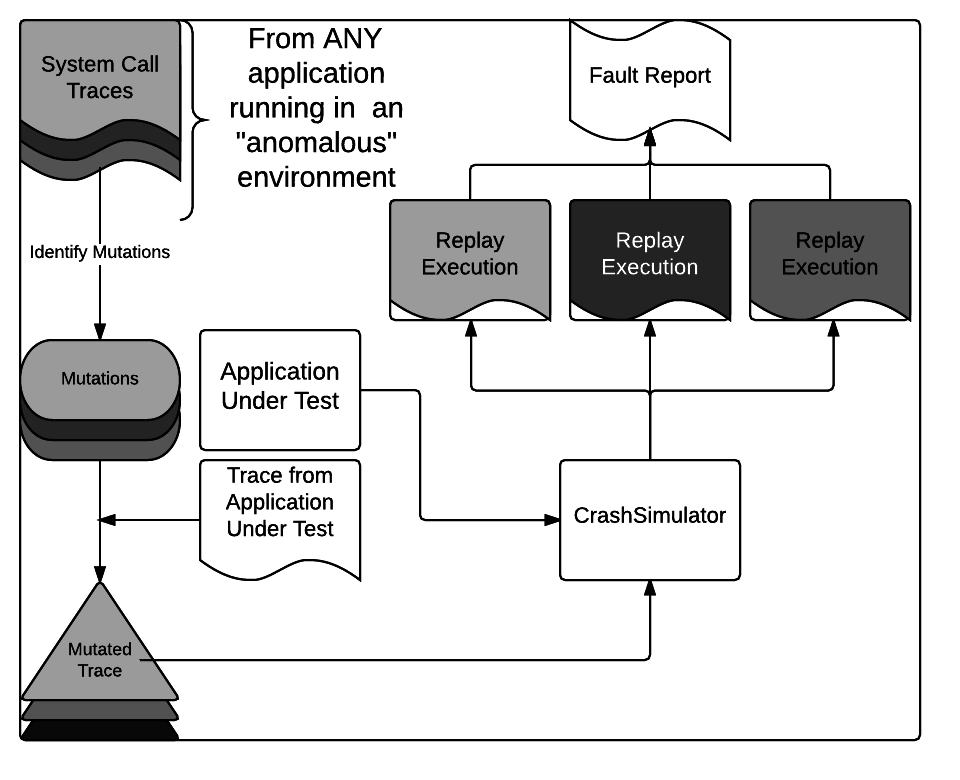
\includegraphics[scale=.5]{Architecture}}
        \caption{\emph{We need a new figure.}}

    \end{figure*}

    \subsection{Architecture}
        
    At a high level CrashSimulator is organized into three primary modules. The first module is responsible for
    monitoring a given execution, determining when to inject anomalous behavior, determining whether or not the
    application responded correctly to the injected behavior. The second module is responsible for managing the
    execution of the application under test such that it precisely follows a previously recorded system call trace -- a
    process we refer to as ``replaying'' a system call trace. The third module orchestrates the process of running
    multiple different anomalies against the application under test, much like a unit test suite.
        
    The first step in CrashSimulator's work flow is to identify anomalous behavior in an arbitrary application. For the
    purposes of this work, this step is accomplished through manual bug hunting and through examination of diagnostic
    output from NetCheck and CheckAPI. CrashSimulator's user examines the system call behavior that resulted in this bad
    behavior and constructs a model defines what triggers the anomalous behavior and the subsequent ``bad'' system call
    behavior (\emph{Do we need to say something about future work doing this step automatically here?}.
    CrashSimulator's first module operates by using this model to analyzed the system call behavior of the application
    under test(e.g. order, parameters, side effects, return values).
        
    CrashSimulator's second module makes use of the Ptrace facilities built into modern versions of the Linux
    kernel. The aforementioned ``replay'' of a system call trace is achieved by intercepting every system call the
    application makes, preventing the actual system call from being carried out by the kernel (i.e. no-oping out the
    real system call, that is replacing it with a call to getpid()), identifying the matching system call from the
    previously recorded trace, and replicating the return value and side effects such that the application believes that
    the system call it made actually took place. We have found that faithfully emulating the post conditions of the
    system calls an application makes results in deterministic replay of a previous execution in most cases.

    Replay is important because it allows CrashSimulator to execute an application free from dependencies on things like
    file system contents, network configuration, or communication with other applications....... \emph{need more here
      -Preston}

    All three primary CrashSimulator modules are packaged together and interact with each other at the appropriate times
    without user intervention. At this point, CrashSimulator itself is available as a virtual machine appliance
    compatible with the \emph{Virtual Box} virtual machine hosting software. The reasons for distributing CrashSimulator
    in this manner are threefold. First, this distribution method ensures that all of CrashSimulator's dependences are
    installed and configured appropriately. Second, this method provides an environment for taking system call traces
    that is known to be complete tool-wise and compatible with CrashSimulator. Finally, and most importantly, this
    method provides an environment that is known to be compatible with the details of CrashSimulator's system call
    replay techniques.

    CrashSimulator's source code is available and, while other environments may be untested, it should function
    correctly on any platforms that meet the criteria described above.

    \subsection{Anomaly Identification}
    
    \emph{This is an old paragraph but I'm leaving it in because I think the general idea it conveys is
      good. -Preston}The first step in CrashSimulator's operation is the analysis of the set of input system call traces
    recorded from other applications running in the intended deployment environment. These traces can be taken from any
    application that as environmental requirements that are reasonably similar to the application under test. For
    example, a web server could likely be effectively tested by CrashSimulator when CrashSimulator is given system call
    traces from other applications that make heavy use of the network. Testing a web browser with traces from an
    application that has no network usage at all would result in less effective testing.
    
    A variety of tools capable of identifying anomalies usable by CrashSimulator already exist. This work relies on
    NetCheck and CheckAPI for this purpose. NetCheck readily able to identify a wide variety of anomalous behaviors
    related to network communication between one or more hosts. During normal operation, NetCheck analyzes a group of
    input system call traces and attempts to produce a diagnosis for network related faults. These faults can be
    analyzed by CrashSimulator's user so that models that encode them can be constructed. CheckAPI peforms a similar
    function by comparing ``behavior of an API implementation to a reference model.''
    
    Additionally, models were constructed that encoded issues identified through manual bug hunting. Specifically,
    we constructed models that identified bad behavior around moving files from one filesystem to another. Using these
    models, CrashSimulator was identify when applications (nodejs etc.) performed this operation incorrectly.

    This process of identifying anomalies does not need to be performed for each run of the test suite.  CrashSimulator
    maintains a corpus of anomalies it has extracted from sample traces. These anomalies can be used to produce mutated
    traces for any future application that it tests. This allows a developer to build up a set of anomalies that were
    identified from each of their target environments. The developer can then test an application against this set of
    anomalies and get an idea of how their application will behave should it encounter the anomalies a deployment
    environment.

    \subsection{System Call Traces}

    \emph{Do we need to keep this justification for using System Call Traces?}
    Where other tools base their operation of direct analysis of the application under test CrashSimulator operates
    based on information gleaned from system call traces. This gives CrashSimulator several advantages over similar
    tools. First, CrashSimulator operates in a language independent manner. It can test any program given two conditions
    hold true:

    \begin{enumerate}
    \item{The application can run in the testing environment}
    \item{System call traces can be recorded from from applications similar to the application under test while
        they run in the intended deployment environment}
    \end{enumerate}

    Utilizing system call traces provides CrashSimulator with two advantages over similar tools. First,
    CrashSimulator has no need for complex language parsing and analysis code. It can test an application regardless
    of the programming language it was written in. Second, while other tools focus on the application under test in
    isolation, CrashSimulator is able to extensively test the interfaces between the application under test and its
    environment. This means that faults resultant from these interfaces are readily identified. For example,
    existing tools are able to quickly test for flaws that result from improper parsing of data once it
    has been received from across a network. CrashSimulator is able to induce and identify flaws that result from
    improper behavior during the network communication itself. This second type of flaw is much more difficult to
    identify replicating the application's intended deployment environment or deploying the application and testing
    it live.
